\chapter{Activity Based Computing}

Add short introduction

\section{Background}
As explained in the introduction, activity based computing is a new computer paradigm that moves focus from application based computer interaction into a higher level computational support for human activities. The paradigm has its outset in clinical work on hospitals, and seeks to aggregate resources to activities, instead of specific applications. An example of such an activity could be the development of our proof of concept. Opening an activity will cause the relevant services and resources to become available to the user, and allow to user to more easily switch between activities and all their associated services and resources. Figure \ref{fig:activitychart} shows an example of the activity "Proof-of-concept development", its associated services and their resources.

\begin{figure}[h!]
  \centering
    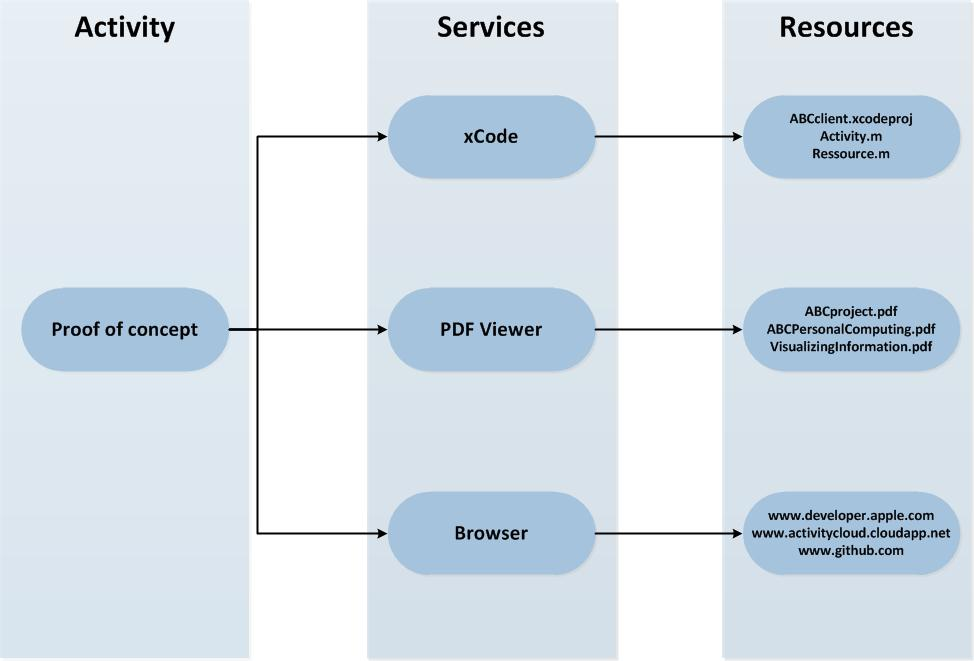
\includegraphics[scale=0.5]{ActivityChart}
  \caption{\emph{The "Proof of Concept" activity. Illustrates how an activity encapsulates its services and resources}}
  \label{fig:activitychart}
\end{figure}

\citet{bardram2011} identifies six principles that forms the basis of the activity based computing paradigm, being; \emph{Activity Centered}, \emph{Activity Suspend and Resume}, \emph{Activity Roaming}, \emph{Acitivty Adaptation}, \emph{Activity Sharing} and \emph{Activity Awareness}. Each of these will be further described in the following.

\begin{description}

	\item[Activity Centered] \hfill \\
	An Activity is a computational unit that encapsulates a set of services and their relevant resources. An activity therefore encapsulate digital software and data necessary for a user to carry out their work (activity).
	
	\item[Activity Suspend and Resume] \hfill \\
	This allows a user to alternate between several activities and support interruptions that requires the user to perform another task. This is done by suspending the current activity and resuming another.
	
	\item[Activity Roaming] \hfill \\
	This principle enables activities to be stored on an infrastructure, like a server, and allows for activities to be suspended on one device, and then resumed on another, to better support user mobility.
	
	\item[Activity Adaptation] \hfill \\
	An activity can be displayed and handled on very different devices, and should adapt to the resources available at the resumed devices. In this case resources could be CPU power, screen size and network bandwidth.
	
	\item[Activity Sharing] \hfill \\
	Focuses and deals with the collaborative aspect of activities. This principle states that activities are shared among collaborators that appear on a list of participants for any particular activity. If two or more participants engage resumes the same activity they will both be notified and engage in video and audio chat if possible.
		
	\item[Activity Awareness] \hfill \\
	Allows for an activity to be context aware, such that it adapts itself to its current environment and work context. This could be to i.e. adapting the user interface or changing activities and services based on where the device is located.

\end{description}

Implementing all of these features enables computational devices to better support human activities, and allow users to move away from the traditional document -and application centered model on a desktop computer.

\section{Activity Adaptation and Awareness}


\section{ABC Framework}

